%% Author_tex.tex
%% V1.0
%% 2012/13/12
%% developed by Techset
%%
%% This file describes the coding for rsproca.cls

\documentclass[]{rsos}%%%%where rsos is the template name

%%%% *** Do not adjust lengths that control margins, column widths, etc. ***

%%%%%%%%%%% Defining Enunciations  %%%%%%%%%%%
\newtheorem{theorem}{\bf Theorem}[section]
\newtheorem{condition}{\bf Condition}[section]
\newtheorem{corollary}{\bf Corollary}[section]
%%%%%%%%%%%%%%%%%%%%%%%%%%%%%%%%%%%%%%%%%%%%%%%


\begin{document}

%%%% Article title to be placed here
\title{Allometric Consumer-Resource Model}

\author{%%%% Author details
Taran Rallings$^{1}$, Justin D. Yeakel$^{1}$} 
% and X. Third author$^{3}$}%

%%%%%%%%% Insert author address here
\address{$^{1}$School of Natural Science, University of California Merced}
% $^{2}$Second author address\\
% $^{3}$Third author address}

%%%% Subject entries to be placed here %%%%
\subject{foodwebs, paleontology, ecology}
https://www.overleaf.com/project/613bc96ff90ad249f6539d97
%%%% Keyword entries to be placed here %%%%
\keywords{foodwebs, mammals, foraging}

%%%% Insert corresponding author and its email address}
\corres{Taran Rallings\\
\email{trallings@ucmerced.edu}}

%%%% Abstract text to be placed here %%%%%%%%%%%%
\begin{abstract}
Main Takeaway points

1) The mass-density relationship represented by Damuth's Law can be approximated with a 2D allometric consumer-resource model that includes starvation dynamics.

2) The magnitude of consumer population density is set by the environmental context of resource growth rates and carrying capacity interacting with fixed internal resource use. The nature/slope of the mass-density relationship in Damuth's Law is set by internal processes of reproduction and resource use regardless of environmental context. 

3) Increases in actuarial mortality rates can radically alter consumer community structure and lead to the exclusion of small-bodied consumers despite having a stronger overall impact on large bodied consumers.  

4) Predation is very cool. 

5) The harvest of consumer populations lowers the maximum body mass of species in a consumer community if the rate of harvest does not decrease with consumer mass. 

\end{abstract}
%%%%%%%%%%%%%%%%%%%%%%%%%%%


\maketitle

\section{Introduction}
What is the background for this paper? 
What are the questions?

(Taran’s stream of consciousness introduction)

The goal of this paper is to understand how multiple sources of mortality interact in determining densities for consumer species and to build a (mostly) mechanistic consumer-resource model that can be extended to look at paleo food webs. The NSM provided a mechanistic framework for thinking about herbivorous mammals and their resources, tying all the consumer parameters to well documented allometric relationships. The limitation of that model is that it tracks two consumer states: full and starved. A second consumer state creates difficulties for parameterizing mortalities over the two states and leads to computational limitations at the complex food-web level. 

The NSM is a particularly useful foundation for paleo food-webs because the mechanistic parameterization is entirely allometric. When building models for paleo-ecosystems a persistent limitation is how to accurately decide on parameter values for interactions you cannot observe or ecosystems that no longer exist or species that are completely extinct. We cannot collect this data from the field so we need to build on known relationships between body-mass and energy for accurate parameterization. \\




\emph{Introduce the NSM}

The two dimensional consumer-resource model used here is a modification of the three dimensional “nutritional-state model”(NSM) (Yeakel et al 2018). In the NSM the consumer, assumed to be a herbivorous mammal, has two states: a full state and a starved state. The full state is capable of reproduction and experiences no mortality. The starved state is not capable of reproduction and faces mortality. The transition rates between the full and starved states are a function of of resource density. More specifically, the transition rates are a function of the proportional fullness of resource carrying capacity. When the resource is at carrying capacity, transitions between the full and starved states become unidirectional, moving from starved to full. When the resource is extinct, the transition term from starved to full drops out, all consumers transition to the starved state, and then die. \\

\emph{Explain the two-dimensional model}

This NSM has been modified by collapsing the full and starved consumer states into a single consumer population. This modification causes the transition rates between the full and starved states to drop out and leave only intrinsic rates of reproduction and mortality. To capture the implicit effects of starvation these reproduction and mortality rates are modified by the resource density as a proportion of it’s carrying capacity. This is structurally similar to the role resource density plays in the NSM serving to modify transition rates between the full and starved states. Here a resource at its carrying capacity means that the consumer can reproduce at it’s maximum rate. As the proportional resource density decreases the effective consumer reproductive rate decreases in the same way. The starvation mortality rate of the consumer is a function of proportional resource density $(1-R/k)$ as well . When the resource is at carrying capacity the starvation mortality term drops out and no mortality by starvation occurs. As proportional resource density is reduced the starvation mortality rate increases. Eventually, at resource extinction $R=0$, the starvation mortality rate reaches its maximum. \\


\emph{Explain how rates are mechanistic}

The vital rates in our model have time scales based on the general ontogenetic growth model in (West et al 2001). The rates vary as a function of the energetics of building and maintaining somatic tissue in both adults and juveniles. Building the model in this way allows us to mechanistically consider the affects of metabolism and by extension of organismal body-size.

*** Explain in more detail in methods. ***


\section{Results and Discussion}


At equilibrium, the allometric consumer-resource model provides an approximation to the mass-density relationship seen in terrestrial herbivorous mammals. The magnitude and slope of this approximation is a product of a few key environmental and physiological variables. The magnitude of the pattern of equilibrium densities is set chiefly by the growth rate and carrying capacity of the resource as well as the starvation rate of the consumer. The slope of the pattern is an interaction between many internal physiological rates, including reproduction and starvation, but is unaffected by resource environment. When sources of mortality beyond starvation are included they can cause deviations from Damuth's Law. This can occur by raising actuarial mortality rates but is most apparent when those mortalities do not themselves mirror the negative scaling pattern with body mass that defines Damuth's Law. The introduction of a non-scaling or positive scaling harvest rate can exclude large bodied consumers completely, leaving a size-depleted consumer community such as is found after the terminal Pleistocene. 

*** cool predation results ***




\subsection{Allometric Consumer-Resource Model}

In the foundational version of the model can be seen below. Eqn 2.1 represents consumer dynamics and eqn 2.2 represents resource dynamics.  

Consumer growth occurs as a function of resource consumption $\frac{R}{0.5k}C$ rates and consumer reproduction $\lambda$. Consumer mortality is a function of resource consumption  $\frac{R}{k}C$ and the starvation rate $\sigma$.

Resource growth occurs by logistic growth and is a function of current resource abundance in relation to carrying capacity  $R(1-\frac{R}{k}C)$ and the intrinsic growth rate parameter $\alpha$. External resource mortality that is not included in logistic growth occurs by interactions with consumers. The per consumer rate of consumption $(\frac{\lambda}{Y}\frac{R}{0.5k} + \rho)$ represents the rate of consumption required for consumer growth $\frac{\lambda}{Y}\frac{R}{0.5k}$ as well as the maintenance rate $\rho$.
\vspace{0.5cm}





\begin{equation}
    \frac{dC}{dt}= \lambda\frac{R}{0.5k}C- \sigma(1 - \frac{R}{k})C
\end{equation}

\begin{equation}
    \frac{dR}{dt} = \alpha R(1 - \frac{R}{k}) - (\frac{\lambda}{Y}\frac{R}{0.5k} + \rho)C
\end{equation}

\vspace{0.5cm}

\subsubsection{Comparison of timescales}
Collapsing this three-dimensional model with explicit starvation to a two-dimensional model with implicit starvation is justified because the time scales at which the dynamics of starvation and recovery occur are significantly faster than the rates at which population dynamics occur. 
*** this needs some actual numbers ***

\subsubsection{Damuth in 2D}

This subsection is a demonstration of the fact that the model produces damuth's law. 

Collapsing the 3-dimensional starvation model into two dimensions maintains the fit of that model to damuth’s law (compare slopes). 

- how is the 2D different than the 3D
0.776818 is this slope\\

A key result of the NSM with explicit starvation is that the population dynamics produce equilibrium consumer densities that closely match Damuth’s Law (*** cite damuth’s law). Our two-dimensional model with implicit starvation also recreates Damuth’s pattern of consumer densities. The greatest deviation of our model from Damuth's law is in small bodied organisms. The CR model overestimates the equilibrium densities of small bodied organisms, possibly through not accounting for predation. This overestimation also has the effect of lowering (steepening) the slope of our mass-density relationship.

(*** what is the actual difference in slope?)


\vspace{0.5cm}

\includegraphics[width=0.8\textwidth]{starvation_damuth.png}

\vspace{0.5cm}








\subsection{The Many Faces of Death}

The fact that our collapsed form of the NSM generates the Damuth pattern is a remarkable result. The objective here is to understand the relationship between the input parameters and the fit to Damuth’s Law. This will help us better understand how the model works, to what degree the pattern is driven by allometric vs environmental forces, and how Damuth's Law may differ for taxa with differing allometries and metabolisms.

To identify the most important relationships in this dynamical view of the consumer-result model that results in Damuth we use correlation plots to see how the fit to Damuth's Law is changed by altering the parameter values. In nature, some of these parameters may be highly plastic and some may be hardwired functions of consumer physiology. Let us first explore without constraints and then look at what is reasonable to expect by environment, taxa, or data limitation. 

(for self – let’s weave a thread of building expectations about what this means for dinosaurs through the paper. Specifically wrt gigantothermic and mesothermic metabolisms but also to very large body sizes. The actual content about this may go at the end but start figuring it out along the way)

\subsubsection{Starvation mortality (foundational, intrinsic, mass-specific, small-size punishing)}

In the equilibrium scenario with starvation as the sole source of mortality, reproduction and mortality rates are equal for all consumer body-masses. As these rates are examined at the system equilibria this matching of rates is by definition and not ecologically interesting.


The figure below is the rates of reproduction and starvation unmodified by resource density. This gives the maximum values for both rates. We can see that in this case the starvation rate, the death rate when no resources are present, as we would expect for a scenario with no resources present. The starvation rate asymptotes at *** find actual value *** but this body mass is well above the largest bodymasses seen in nature among terrestria mammals *** insert deinothrere/indricothere reference *** \\

\vspace{0.5cm}

\includegraphics[width=0.9\textwidth]{starvation_reproductionrates.png}\\

\vspace{0.5cm}

\emph{Correlations} 

The consumer-resource equation form with starvation as the only form of consumer mortality is used to generate the slope and y-intercept correlation figures. Slope and y-intercept here refer to the line fit to generated data on a graph of consumer population density by body-mass. This is the style of graph used to demonstrate Damuth’s Law and that pattern is replicated here in order to compare our model results to that law. 

*** I'll need to redo the following in a longer run but for now... ***
The correlations were generated over 5000 runs of the consumer-resource model. In each of these runs the parameters are randomized by a factor between 0.5 and 1.5. The resulting mass-density relationship is expressed as a linear model and Pearson’s correlations are run for the relationship between the parameters and either the linear model slope or y-intercept. \\

\vspace{0.5cm}
	
\includegraphics[width=0.9\textwidth]{slope_corr_starv.pdf}

\vspace{0.5cm}

The slope of the Damuth line represents the strength of the negative relationship between species’ body mass and the population density of that species in the environment. 


The resource parameters, $\alpha$ and \emph{k}, are not correlated with any change in the slope of the Damuth line. While we would expect resource conditions to affect the value of the population density they are not themselves functions of consumer mass and so do not affect the distribution of density changes across body masses.


$\lambda$, the reproductive growth rate of the consumer, has a strong negative effect on the slope of the Damuth line, making the relationship between consumer mass and density steeper. The higher $\lambda$ is, the more dramatic the reduction in population density as body mass increases. If comparing large body mass consumers, the consumer with higher reproductive growth rate will exist at lower population densities than the one with a lower growth rate. This can occur by increasing the fecundity of the species or reducing the timescale of reproduction. 
 $\lambda$ appears in the mortality term for the resource so as it increases so too does the mortality of resources. As the rate of reproduction is increased more energy is being shunted to generating young, reducing resource density.



\emph{Y}, $\rho$, and $\sigma$ are positively correlated with the slope of the Damuth line. This means that as these parameters are increased, the mass-density relationship becomes shallower and equilibrium population densities look more similar across body-masses. 

The yield coefficient, \emph{Y}, represents a conversion efficiency from resource to consumer. It is the units of consumer produced per unit of resourced eaten. As yield is increased, less energy is lost during consumption. This means that fewer resources are eaten per consumer and higher consumer densities can be maintained. 

$\rho$, is the maintenance rate of resource consumption. This rate is in units of resource per second per unit of consumer. It is the amount of resource that must be consumer per second to maintain a unit of consumer. As $\rho$, is increased the slope of the Damuth line becomes shallower because the metabolic efficiencies of large body-mass are felt more strongly the larger $\rho$, becomes. 

$\sigma$ is the maximum starvation mortality rate experienced by consumers when the resource is absent.  Under conditions where the resource is present the consumer experiences some portion of the starvation rate depending on the current proportion of carrying capacity currently satisfied by the resource density. $\sigma$ is positively correlated with the Damuth slope, the lines becomes shallower as $\sigma$ is increased. This suggests that as starvation becomes a stronger force on populations the differences in metabolic efficiency between large and small organisms are overwhelmed, resulting in more similar population densities. \\

\vspace{0.5cm}

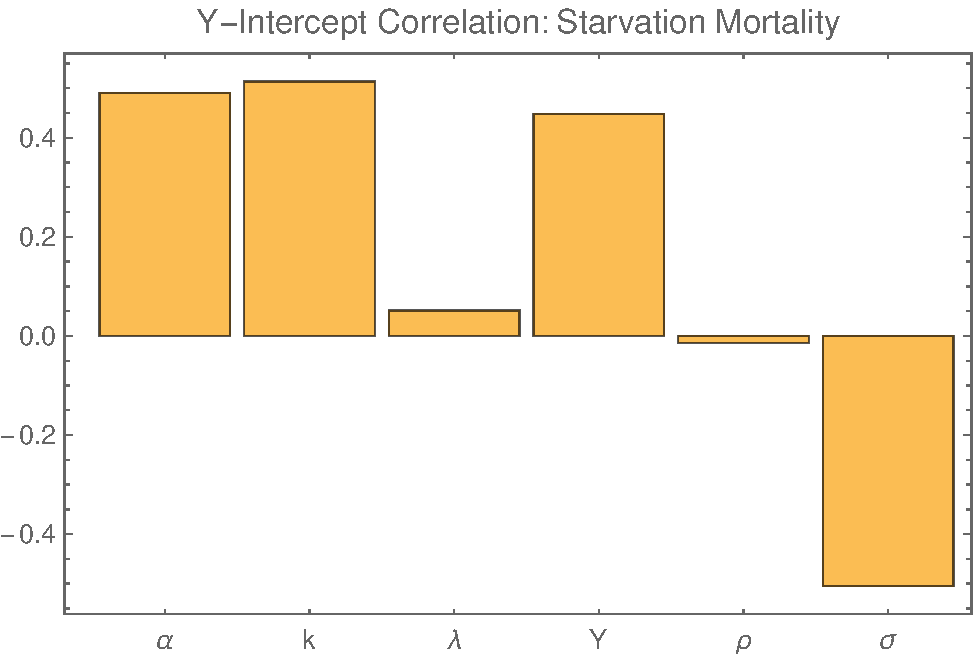
\includegraphics[width=0.9\textwidth]{int_corr_starve.pdf}

\vspace{0.5cm}

\emph{Y-Intercept Correlation}

The y-intercept of the Damuth line represents the magnitude of the density for the hypothetical zero-mass consumer. While the slope gives us information on the mass-density relation over a range of masses, the intercept sets the scale over which that relationship occurs. A positive correlation means a parameter increases population densities , a negative correlation means a parameter decreases population densities. 

$\alpha$ and \emph{k}, the resource growth rates and carrying capacity, are both positively correlated with the intercept. This makes sense because they are both parameters indicating resource abundance in a system. A high $\alpha$ means the resource is productive and quickly renewing. A high \emph{k} means the resource can exist in great abundance. Both scenarios provide more food for consumers which leads to higher population densities.

$\lambda$, the consumer growth rate, has little to no effect on the intercept. Increasing the pace of reproduction does not increase the maximum supported population in a system in which consumers face resource limitation, like this model. 

The yield coefficient, \emph{Y}, represents a conversion efficiency from resource to consumer. It is positively correlated with the intercept. A high conversion efficiency will have an effect similar to increasing resource abundance because the effective abundance of the resource is increased when fewer resources need to be consumed to grow one unit of consumer.

$\rho$, the consumer maintenance rate, has little effect on the intercept of the fit to Damuth's Law. *** not currently clear to me why this is the case. Rho is actually at it's highest value at the Y intercept. I need to think about this some more  ***

$\sigma$ has a strong negative correlation with the intercept. In this version of the model, starvation mortality is the sole source of death for consumers. It plays a strong role is setting equilibrium densities for both resources and consumers. This makes sense as the equilibrium of a population is principally a function of the balance of birth and death processes. So as mortality is increased the equilibrium density of the consumer is decreased. \\
	
	
	

\subsubsection{Survivorship mortality (intrinsic, mass-specific, small-size punishing))}



\begin{equation}
    \frac{dC}{dt}= \frac{\lambda}{0.5k}RC- (\mu+\sigma)(1 - \frac{R}{k})C
\end{equation}

\vspace{0.5cm}

\begin{equation}
    \frac{dR}{dt} = \alpha R(1 - \frac{R}{k}) - (\frac{\lambda}{Y}\frac{R}{0.5k} + \rho)C
\end{equation}


\emph{Reproduction, Starvation, and Survivorship}

 Survivorship mortality, in its form containing both initial cohort mortality and actuarial mortality, has a steeper slope than survivorship mortality. This means it is more harmful to small bodied organisms than large bodied organisms. This has the effect of bringing small and large bodied consumer equilibrium population densities closer to together in size. The principle components of survivorship are initial cohort mortality and actuarial mortality. (cite Calder for all this stuff)\\



\includegraphics[width=0.9\textwidth]{survivorship_rates.png}\\

\vspace{1.0cm}


\emph{Initial Cohort Mortality}

Initial cohort mortality (or initial vulnerability) sets the fundamental the rate of disappearance of individuals from a population. As initial cohort mortality is increased or decreased the magnitude or mortality changes for all body masses but the slope of that relationship between mass and mortality does not change. \\

\vspace{0.5cm}

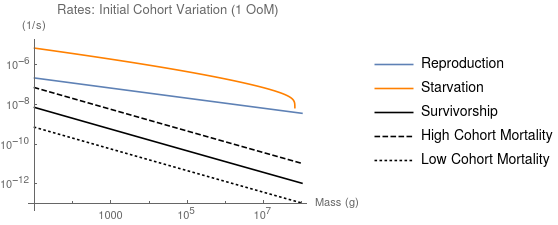
\includegraphics[width=0.9\textwidth]{cohort_plot.png}\\ 

\vspace{0.5cm}

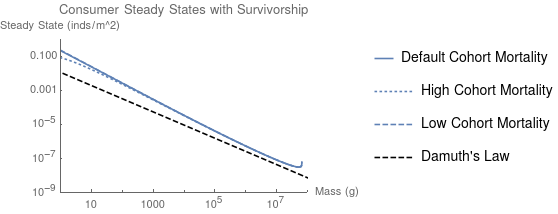
\includegraphics[width=0.9\textwidth]{cohort_damuth_plot.png}\\ 
\vspace{0.5cm}

In order for survivorship mortality to approach reproduction in value through a change in initial cohort mortality it must be raised at least one order of magnitude. Even under this conditions of dramatically increased mortality it is still only for the  small bodied organisms that survivorship begins to rival reproduction rates because the slope of survivorship is steeper than reproduction\\

\emph{Actuarial Mortality}

For most species, mortality rates increase over time with the age of individuals. Actuarial mortality is a measure of that increase in mortality rate in a cohort as that cohort ages. As actuarial mortality is changed the magnitude of mortality increases but the slope changes as well. Increasing actuarial mortality decreases the slope of the mass-mortality relationship because larger organisms live longer and so are more effected by the cumulative build up of mortality that occurs via actuarial mortality rates.\\

\vspace{0.5cm}

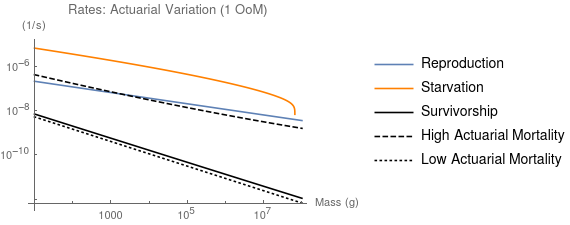
\includegraphics[width=0.9\textwidth]{actuarial_plot.png}\\ 

\vspace{0.5cm}


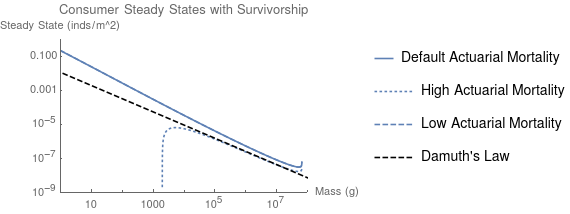
\includegraphics[width=0.9\textwidth]{actuarial_damuth_plot.png}\\ 

\vspace{0.5cm}

Increasing the actuarial mortality rate by an order of magnitude overwhelms the reproduction of small bodied organisms but also comes close to overwhelming the large bodied reproduction rates as well. Were an ecological context to arrive that dialed up the actuarial rate the community would be defaunated by size class from small to large. \\


\subsubsection{Predation Mortality (extrinsic, mass-specific, small-size punishing)}

explain what it is and how it works 
	
reproduction and mortality rates figure
	
discussion the results of these figures and interpret


\subsubsection{Harvesting Mortality (extrinsic, mass-non-specific, large-size punishing)}

\vspace{0.5cm}


\begin{equation}
    \frac{dC}{dt}= \frac{\lambda}{0.5k}RC- (\xi+\sigma)(1 - \frac{R}{k})C
\end{equation}

\vspace{0.5cm}

\begin{equation}
    \frac{dR}{dt} = \alpha R(1 - \frac{R}{k}) - (\frac{\lambda}{Y}\frac{R}{0.5k} + \rho)C
\end{equation}


\vspace{0.5cm}

In the scenario where mortality includes a harvesting rate, the resulting patter is quite different. Size-blind harvesting places the same magnitude of mortality pressure on all consumers. The nature of the allometric scaling of reproduction means that large bodied organisms reproduce much more slowly than small bodied organisms. Sources of mortality like starvation and survivorship follow this same pattern, placing the strongest mortality pressures on small bodied organisms. 

As harvest is an external mortality source placed on a population, here using harvest by humans as the guiding example, the manner in which it scales with consumer body-mass can vary. Here we examine three scenarios of harvest rate and their effects: non-scaling, positive scaling, and negative scaling. \\

\vspace{0.5cm}

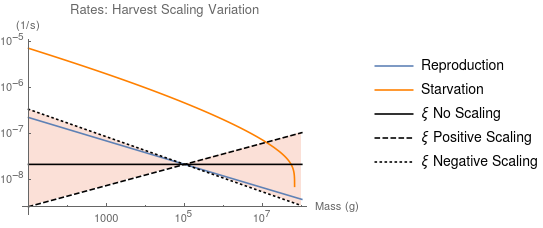
\includegraphics[width=0.9\textwidth]{harvest_scaling_plot.png}\\

\vspace{0.5cm}

Non-scaling - A harvesting rate being blind to consumer mass breaks the pattern of decreasing rate with mass and can drive large bodied organisms to extinction as the harvesting rate, combined with starvation and other sources of mortality, overwhelm the reproductive capacity of the species. The effect on the Damuth line is to lower the maximum body-mass of species facing the harvest pressure.\\

\vspace{0.5cm}

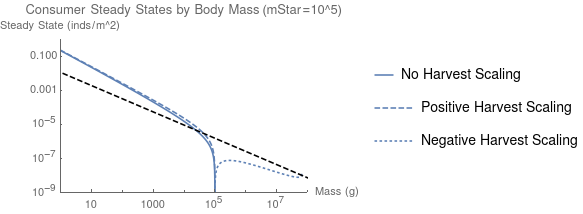
\includegraphics[width=0.9\textwidth]{harvest_damuth_plot.png}\\

\vspace{0.5cm}

In the figure above we can see that large-bodied consumers are excluded from the system, harvesting pressure overwhelms the reproductive capacity. This result is qualitatively similar for the positive-scaling harvest scenario as well as the non-scaling scenario.


Positive scaling – A harvesting rate with positive scaling maintains the basic pattern of a non-scaling harvest rate. Large bodied consumers face a higher mortality relative to their reproduction rates and so face extinction at lower harvesting rates than do small bodied organisms. This can represent hunting styles and technologies that prioritize large bodied prey, such as clovis points and atlatls.  The effect on the Damuth line is to lower the maximum body-mass of species facing the harvest pressure.\\

Negative scaling – A harvesting rate with negative scaling inverts the pattern of the other scaling approaches and behaves more like starvation and survivorship, having higher mortalities for small bodied consumers. This pattern could occur under hunting regimes that emphasize trapping. This can create situations where only large bodied consumers can survive in the ecosystem, all small-bodied consumers having gone extinct from the combined weight of harvest and intrinsic mortalities. \\


In the figure above we can see the negative scaling has excluded small bodied consumers from the system. Large bodied consumer equilibria persist in a narrow band of density between zero and the starvation-only scenario, leaving them vulnerable to stochastic events. 

\vspace{1.0cm}

Predicting values of harvest:

This section is not actually written yet but this is the raw material. We can see whether it'll be useful or not after the earlier sections are ironed out. 

(this stuff is from dimensionality of predation). 
Encounter rate with a human population sets the maximum harvest rate for unfocused (random encounter) harvest. At the levels of population density predicted for Pleistocene Africa, these random encounters would be insufficient to drive any species extinct even if all encounters were successful harvesting events. 
This conception of population density is an average over large swaths of land and does not account for the clumping of human population densities within hunting territories. \\

\vspace{0.5cm}

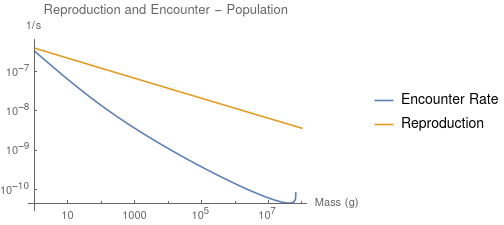
\includegraphics[width=0.9\textwidth]{pop_encounter_plot.png}\\

\vspace{0.5cm}

As human population density is increased, the rate of encounter overwhelms the reproduction of small bodied animals. The pattern of these interactions is in line with the expectation of a negative scaling on harvest rate. This suggestions \\

\vspace{0.5cm}

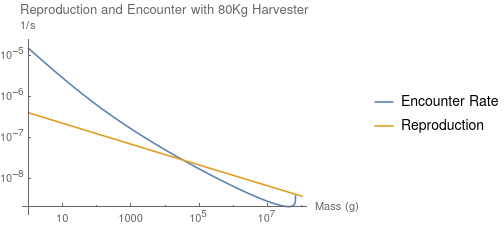
\includegraphics[width=0.9\textwidth]{encounter_plot.png}\\

\vspace{0.5cm}


% \noindent \textbf{Resource Landscape:} 



% \noindent \textbf{Resource Traits:}







% \noindent \textbf{Herbivore Traits:}




%Parameterization

%Justification



\section{Methods}

 include detailed parameter stuff and derivations

- explain the foundation of the 3D model from the starvation paper

- explain the collapse to 2D, how it was done and why it works

- explain, in detail, where on earth all of these parameters come from

- explain the role of resource carrying capacity in the consumer dynamics

- justify under what conditions the k thing makes sense and where it doesn’t

- explain the methods of analysis – analytical, simulation, and population dynamics

- explain how the relationship between parameters and real resources/herbivores was done

- explain how the new survivorship mortality works

- explain how the new starvation mortality works

- explain how the new harvesting mortality works

- explain how the new predation mortality works

\vspace{0.5cm}

\emph{Explain the basic parameters of the model}

$\lambda$ is the maximum consumer reproduction rate (1/s) under ideal resource conditions. Structurally, its form is ln(2)/Tlam. The fecundity of the consumer is given by the logged number in the numerator, 2 in this case. Tlam is the time from reproductive event to maturity for an organism of a given bodymass. 


$\mu$ is the survivorship mortality rate. This is a representation of a variety of mechanisms to meet misadventure that are mass-dependent but exclude explicit predation. The value is derived from the Gompertz equation. (review details to write details)

$\emph{Y}$ is the yield coefficient – the number of units of organism that are produced per unit of resource that is consumed. Yield is a function of consumer body mass and resource energy density.

$\rho$ is the consumer somatic growth rate (1/s). In the NSM this served as a “rate of recovery” that governed transitions from the starved to full states. Here it is a maintenance parameter that sets part of  resource consumption without adding to consumer growth. 

$\alpha$ is the specific growth rate of the resource (1/s). This is a function of bodymass and resource energy density

\emph{k} is the resource carrying capacity. The value is set empirically. It is important to note that the specific meaning of k in this model is complicated. In addition to the standard lotka-volterra usage in the resource equation for logistic growth, k is used as a modifier on consumer growth and mortality terms.

Consumer growth rate is expressed with lambda * (R/k). This means that the proportion of consumer growth rate that is expressed is 1:1 with the proportion of resource carrying capacity that is realized at that time. The model assumes that k represents a resource density whereby the consumer experiences no resource limitation. Because of this the relationship between the consumer, the resource, and the resource carrying capacity need to be carefully thought out in parameterization. For most consumer-resource pairings this assumption, and thereby model, will fail. 


$\sigma$ is the consumer starvation rate. This starvation rate is a function of consumer body-mass, through allometric equations for the time to starvation from a full state. 

Similarly to the modification of consumer growth rate, the starvation mortality rate is modified by the realized proportion of resource carrying capacity. The rate sigma is multiplied by (1-R/k). This follows the previous assumption that a consumer experiences no resource limitation if the resource is at carrying capacity. When R=k, starvation mortality drops to zero. When R=0, starvation is maximized.  The same care must be applied here as with k in growth. The model assumes that the value of k for a given resource is sufficient to remove entirely the risk of starvation for consumers.

$\xi$ is the extrinsic consumer mortality rate (1/s). This is meant to represent sources of mortality that are blind to consumer body-mass such as harvesting by humans and environmental catastrophes (*cough* meteors /*cough*). The extrinsic mortality rate modifies consumer density only. A density independent extrinsic mortality rate could be added but it’s use cases are less obvious. The interaction of this parameter and the intrinsic mass-dependent sources of consumer mortality are of central interest in this study.  

\section{Discussion}


\section{Conclusion}
The conclusion text goes here.

\vskip1pc

\ethics{Insert ethics text here.}

\dataccess{Insert data accessibility text here. '(If no information, then please include the text ``This article has no additional data'').}

\aucontribute{Insert author contributions text here (to be included if more than one author).}

\competing{Insert competing interests text here.}

\funding{Insert funding text here.}

\ack{Insert acknowledgment text here.}

\disclaimer{Insert disclaimer text here.}


\pagebreak

%%%%%%%%%% Insert bibliography here %%%%%%%%%%%%%%
\bibliographystyle{RS}
\bibliography{aa_starving3}

\end{document}
